\chapter{Introduction}\label{introduction}
\fxnote{Previous version: ``We, the group 630 on the Bachelors Degree in Control, wanted to work with an unstable system for this bachelor project in control engineering. The choice fell on a form of inverted pendulum setup that is called Cubli.''} 
Effective control of inverted pendulum is still an active area of research nowadays \cite{JHuber}.\\ %Choosing such a system as a Bachelor project in Control Engineering is therefore a stimulating but acceptable challenge\fxnote{find synonym for stimulating, and reword the challenge thing, B}.\\
One type of inverted pendulum is a setup called Cubli. It consists of a cube controlled with reaction wheels. The Cubli can jump up and balance on one of its edges or on one of its corners, as shown in \figref{CubliCorner}.
The Cubli is designed as a simple setup to let control engineers work with an inverted pendulum. A working Cubli can also be an interesting thing to show the general public and explain what control engineering is about.  \cite{MGajamohan}

\begin{figure}[H] 
	\centering
	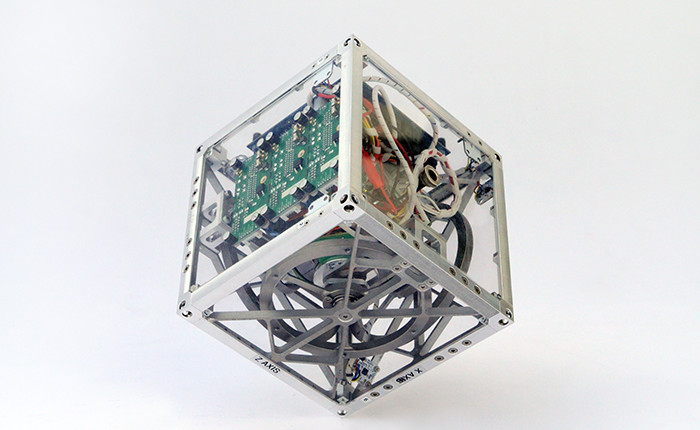
\includegraphics[scale=1.3]{figures/CubliCorner-700x430}
	\caption{A Cubli balancing on one of its corners\cite{RAndrea}}
	\label{CubliCorner}
\end{figure}
Applications for this cube robot, that moves without any external tools, might seem limited when you only have a single cube. However, if you take a group of cubes, they could move together to traverse obstacles or solve puzzles one cube alone could not. A group of cubes can form a structure (\figref{MBlocksExample}), and by talking in between each other they can use their reaction wheels to get the structure to move in the desired direction. Since each cube can move independently, a single cube can detach for an assignment or catch up with the main structure if it gets dropped.\cite{JRomanishin}

\begin{figure}[H] 
	\centering
	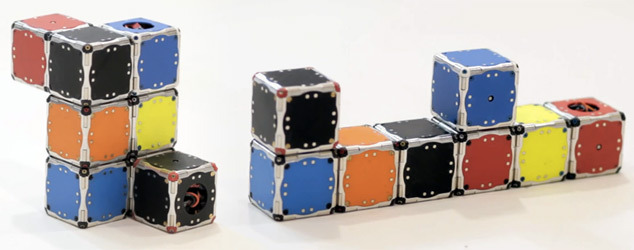
\includegraphics[scale=0.4]{figures/m-blocks}
	\caption{A number of cube robots (called M-blocks at Massachusetts Institute of Technology (MIT)) shown making two different structures. These M-blocks stick together with the help of magnets placed in their corners\cite{LRosen}}
	\label{MBlocksExample}
\end{figure}